\section{Server}

\subsection{Was ist ein Server?}
Als \textit{Server} eng(Diener) wird sowohl ein Computer mit einem Netzwerk genannt,
als auch ein Programm, das auf diesen Pc läuft. Somit gibt es also \textbf{zwei} Definitionen
für einen Server.

\subsubsection{Server (Hardware)}
Als Hardware Server wird ein Rechnernetz aus einem Computer, auf dem neben dem Betriebssystem
mehrere softwarebasierte Server laufen. Bezeichnet wird ein solcher hardwarebasierter
Server als \textbf{Host} (englisch für Gastgeber). Jeder Rechner kann im Prinzip als Host verwendet
werden.

\subsubsection{Server (Software)}
Ein software Server ist in der Regel ein Programm oder ein Anwendung
der von anderen Rechnern den sogenannten Clients lokal über ein Netzwerk in Anspruch genommen
werden kann. Die Art der Server der Server Software bestimmt den Dienst des Servers. Grundlage für
eine Kommunikation bildet das Client-Server-Modell. \ref{db}

\subsubsection{Funktionsweiße eines Servers}
Wie bereits erwähnt basiert die Kommunikation zwischen den Server und den Clients
auf der Grundlage des \textit{Client-Server-Modells}. Jeder Dienst der, im Netzwerk wird von
einem dauerhaft erreichbaren Server zur Verfügung gestellt. Somit kann sichergestellt werden, dass
Dienste wie Webbrowser E-Mail zu jeder Zeit auf den Server zugreifen können um den Dienst
in Beanspruchung nehmen zu können.

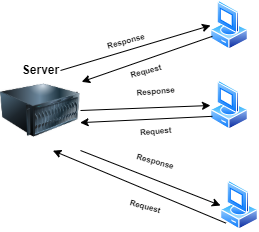
\includegraphics[width=0.50\textwidth]{Backend/client server.drawio.png}
\subsubsection{Welche Arten von Servern gibt es?}
\paragraph*{Webserver}
Ein Webserver hat die Aufgabe, Websites zu speichern, aufzubereiten und an die Webbrowser bzw. Clients
auszugeben. Kommuniziert wird zwischen Server und Software mittels \textbf{Hypertext Transfer Protocol
    (HTTP)} bzw mittels der verschlüsselten Variante \textbf{HTTPS}. Die gängigsten Webserver sind
Apache HTTP Server, Microsoft Internet Information Services (IIS) oder Nginx.

\paragraph{File-Server}
Ein File Server hat die Aufgabe zur zentralen Speicherung von Dateien, welche von den Clients
über ein Netzwerk zugänglich gemacht werden. Ein File Server ermöglicht aufgrund von verschiedenster
Dateiversionen Konflikte entgegenzuwirken. Außerdem erfolgt eine automatische Versionierung der
Daten sowie ein zentrales Back-up sämtlicher Daten. Falls der Zugriff auf den Server über das
Web läuft kommen Protokolle wie \textbf{FTP} (File Transport Protocol), \textbf{SFTP}(Secure File Transfer
Protocol). \textbf{FTPS}(FTP over SSL) oder \textbf{SCP}(Secure Copy) zum Einsatz. Im lokalen
Gebrauch sind die Protokolle \textbf{SMB}(Server MEssage Block) und \textbf{NFS}(Network File System).

\paragraph{Mailserver}
Wie des Name es bereits andeutet ermöglicht ein Mail Server E-Mails zu empfangen, zu senden und
weiterzuleiten. Er besteht aus mehreren Software-Modulen. Zum Einsatz kommt hier in der Regel
das \textbf{Simple Mail Transfer Protocol}(SMTP). User die einen Mail-Server nutzen
wollen benötigen einen E-Mail Client, der die Nachrichten vom Server holt und im E-Mail-Postfach
darstellt. Ein solcher Abruf erfolgt über \textbf{IMAP}(Internet Message Access Protocol) oder
\textbf{POD} (Post Office Protocol).

\paragraph{Datenbank-Server}
Ein Datenbank-Server auch genannt \textbf{Backend-Server} ermöglicht es Programme, über ein Netzwerk,
zugriff auf ein oder mehrere
Datenbanksysteme zu gewährleisten. Die wohl bekanntesten Software-Lösungen sind \textit{Oracle},
\textit{MySql}, \textit{Microsoft SQL Server}, \textit{PostgreSQL} und \textit{DB2}. Um mit dem
Backend Server kommunizieren zu können benötigt der User das sogenannte \textbf{Frontend}.
\ref{db}

\paragraph{Proxy-Server}
Ein Proxy-Server dient als Kommunikationsschnittstelle in einem Rechnernetzwerk. Er nimmt Anfragen
aus dem Netzwerk entgegen und leitet diese über seine IP-Adresse weiter. Eingesetzt wird ein solcher
Proxy-Server um Kommunikationen zu filtern, Bandbreite zu kontrollieren, Verfügbarkeit durch
Lastverteilung zu erhöhen um Daten zwischenzuspeichern auch \textbf{Caching} genannt. Mithilfe eines
Proxy-Servers ist es ebenfalls möglich Anonymität zu gewährleisten, da die IP-Adressen der Clients
hinter dem Proxy verborgen bleiben.

\paragraph{Game-Server}
Ein Game-Server ist ein Server der speziell für onlinebasierte Multiplayer-Spiele entwickelt wurde.
Die Daten des Online Spiels werden verwaltet und somit ist eine synchrone Interaktion mit der
virtuellen Welt möglich. Die Hardware für einen solchen Server kann in einem Rechenzentrum oder lokal
bereit gestellt werden.

\paragraph{DNS-Server}
DNS-Server haben die Aufgabe als Namensauflöser in einem Netzwerk zu dienen. Sie sind also dazu
zuständig das sie Hostename wie www.skate-buddy.com in die entsprechende IP-Adresse übersetzten.

\subsubsection{Server Hosting}
Da das Anschaffen der Server Hardware durchaus teuer werden kann lohnt es sich für Privatpersonen,
die ein eigenes Server Projekt realisieren möchten auf gemietete Ressourcen zurückzugreifen.
Verschiedensten Hosting-Modelle werden von spezialisierten Provider angeboten, dadurch müssen sich
die Benutzer nicht mehr um den Betrieb der Hardware zu kümmern.

\cite{Server}



\label{server}